\documentclass[letterpaper]{l3doc}

\usepackage[mono = false]{libertine}
\usepackage{geometry,pdfpages,tikz,tabularx,xfrac,hologo,authblk}
\hologoFontSetup{general = \sffamily}
\newenvironment{example}{\begin{list}{}{\leftmargin=3em}\item }{\end{list}}
\fvset{xleftmargin = \parindent}
% \usepackage[fontset = none]{ctex}
\linespread{1.15}
\usepackage{indentfirst}
\setlength{\parindent}{2em}
\usepackage[os = mac]{menukeys}

\title{
    The \cls{litetable} Class: Colorful Timetable
    \thanks{\url{https://github.com/xiamyphys/litetable}}
}

\author{Mingyu Xia, Hangzhou Dianzi University}

\affil{\href{mailto:xiamyphys@gmail.com}{xiamyphys@gmail.com}}

\date{Version 3.0B, \today}

\begin{document}

\maketitle

\begin{abstract}
    This is the manual for \cls{litetable} class, which provides a design of timetable with colorful course blocks. Welcome to feedback bugs or ideas via email \href{mailto:xiamyphys@gmail.com}{xiamyphys@gmail.com} or \href{https://github.com/xiamyphys/litetable/issues}{GitHub}. This manual is available in three versions: \textbf{English}, Chinese, and Cantonese.
\end{abstract}

\section{Introduction}

\subsection{Packages required}

This class is based on the \cls{article} class. It requires \pkg{expl3}, \pkg{xparse}, \pkg{tikz}, \pkg{listofitems}, and \pkg{xcolor} packages. 

\subsection{Compatibility}

The required version of the \pkg{expl3} package should support ``e-type'' variants, so it cannot run on the version of \hologo{TeX}Live 2023 or earlier. The test platforms are macOS 15.1 / Overleaf / Ubuntu 22.04.2 with \hologo{TeX}Live 2024 distribution. They all work fine for \hologo{pdfLaTeX} and \hologo{XeLaTeX} compilers. Windows and Unix platforms' compatibility is unknown.

\section{Usage}

\subsection{Loading \cls{litetable} and generate the timetable frame}

Just like loading any class, write

\begin{Verbatim}
    \documentclass{litetable}
\end{Verbatim}

The following commands need the \cmd{tikzpicture} environment with \cmd{remember picture, overaly} option.

\subsubsection{The \cs{maketable} command}

\begin{example}
    \cs{maketable}\oarg{semester}\marg{title}
\end{example}

This command has two arguments that can create an empty timetable frame. The first optional argument can add the semester block at the northeast corner of the page, the second mandatory argument can assign the title.

\subsubsection{The \cs{more} command}

\begin{example}
    \cs{more}\marg{comment}
\end{example}

This command can add a comment at the southwest corner of the page.

\subsubsection{The \cs{timelist} command}

\begin{example}
    \cs{timelist}\oarg{rows}\marg{time list}
\end{example}

This command has two arguments, the first optional argument \oarg{\#1} can directly assign the number of rows on the timetable, and the second mandatory argument \marg{\#2} can add time to the left side of the timetable. Format for inputting array is the following: separate the start time and the end time with a dash (-) and separate the time groups with a comma (,). For example

\begin{Verbatim}
    \timelist[13]{%
        08:05 - 08:50, 08:55 - 09:40, 10:00 - 10:45, 10:50 - 11:35,
        11:40 - 12:25, 13:30 - 14:15, 14:20 - 15:05, 15:15 - 16:00,
        16:05 - 16:50, 18:30 - 19:15, 19:20 - 20:05, 20:10 - 20:55,
    }
\end{Verbatim}

For different usage scenarios of the two arguments, \cls{litetable} will generate a corresponding row-based timetable frame according to the following rules.

\begin{table}[htbp]
    \centering
    \begin{tabularx}{\linewidth}{c X X}
      \toprule
        $\displaystyle\sfrac{\oarg{\#1}}{\marg{\#2}}$ &
        \multicolumn{1}{c}{To use} &
        \multicolumn{1}{c}{Not to use}\\
      \midrule
        To use &
        The effect is the same as described in \marg{\#2}, but the number of rows in the timetable is determined by \oarg{\#1} &
        The effect is the same as described in \oarg{\#1}\\
      \midrule
        Not to use &
        The effect is the same as described in \marg{\#2} &
        ERROR!\\
      \bottomrule
    \end{tabularx}
\end{table}

\begin{itemize}
    \item If the mandatory argument \marg{\#2} receives $X$ sets of time, and the optional argument \oarg{\#1} receives a value of $X+a$, then only lines $1\sim X$ on the left side of the timetable display the time, while the other lines do not display the time.
    \item If the mandatory argument \marg{\#2} receives $X+a$ sets of time, and the optional \oarg{\#1} receives a value of $X$, then there will generate a timetable with only $X$ rows with extra time sets ignored, and it will return a warning.
\end{itemize}

\subsubsection{The \cs{weeklist} command}

\begin{example}
    \cs{weeklist}\oarg{default weeks}\marg{week list}
\end{example}

This command has two arguments. The first optional argument can determine the default number of weeks and print at every course block's southeast corner. The second mandatory argument can add workdays with corresponding width ratios at the top of the timetable. The first line of the input array is the formats of the working days, and the second line is the corresponding width ratio. Two lines are separated by a semicolon (;). For example

\begin{Verbatim}
    \weeklist[Weeks 1 - 16]{%
        \scshape Mon,    \scshape Tue,     \scshape Wed,
        \scshape Thu,    \scshape Fri;     4,5,4,6,5
    }
\end{Verbatim}

\begin{figure}[!ht]
    \centering
    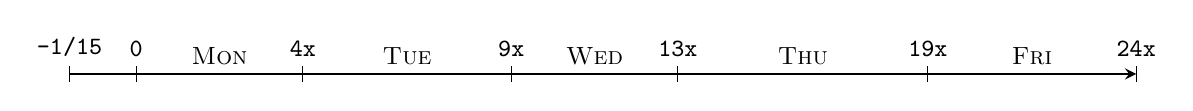
\begin{tikzpicture}[every node/.style={font=\small\sffamily\scshape}]
        \draw [thick,->,>=stealth] (-5 in/15,0) -- (5 in,0);
        \draw (-5 in/15,-.1) --++ (0,.2) node [above] {\verb|-1/15|};
        \draw (0,-.1) --++ (0,.2) node [above] {\verb|0|};
        \draw (4*5 in/24,-.1) --++ (0,.2) node [above] {\verb|4x|};
        \draw (9*5 in/24,-.1) --++ (0,.2) node [above] {\verb|9x|};
        \draw (13*5 in/24,-.1) --++ (0,.2) node [above] {\verb|13x|};
        \draw (19*5 in/24,-.1) --++ (0,.2) node [above] {\verb|19x|};
        \draw (5 in,-.1) --++ (0,.2) node [above] {\verb|24x|};
        \node [above] at (2*5 in/24,0) {Mon};
        \node [above] at (6.5*5 in/24,0) {Tue};
        \node [above] at (11*5 in/24,0) {Wed};
        \node [above] at (16*5 in/24,0) {Thu};
        \node [above] at (21.5*5 in/24,0) {Fri};
    \end{tikzpicture}
\end{figure}

Now, the default value of the key \keys{weeks} is set to \cmd{Weeks 1 - 16}. If the number of workdays is larger than the ratios you input, then the extra workdays will be ignored and it will return a warning.

\subsection{Add course blocks}

Using the \cs{course} command to add course blocks on the current workday. This command has two arguments.

\begin{example}
    \cs{course}\oarg{keyvals}\marg{class start number}\oarg{class end number}
\end{example}

The first optional argument accepts the following keys: \keys{color} \keys{subject} \keys{location} \keys{teacher} \keys{weeks}. The default value of the key \keys{color} is \cmd{DarkSlateGray}, and the default value of the key \keys{weeks} is determined by the first argument of the command \cs{weeklist}. The second and third mandatory arguments are the start and end numbers of the course, respectively. The following is a use case of the command \cs{course}

\begin{Verbatim}
    \course [ color = DarkGreen, subject = listofitems, 
              location = French, teacher = Christian Tellechea
            ] {10} {12}
\end{Verbatim}

\begin{center}
    \noindent\fbox{
        \parbox{.94\linewidth}{\footnotesize
            Set the color of this course block to \cmd{DarkGreen}, the course name to \cmd{listofitems}, the class location to \cmd {French}, and the teacher to \cmd{Christian Tellechea}, starting from the \cmd{10}th class of the day and ending from the \cmd{12}th class of the same day.
        }
    }
\end{center}

\begin{itemize}
    \item One can switch to the next workday via the command \cs{newday}.
    \item If the course block's height is only one unit, that is $\marg{class start number} = \marg{class end number}$, the values of keys \keys{location} and \keys{teacher} will print on the same line with a comma (,) separated, and the value of the key \keys{weeks} will not be printed.
    \item If neither the key \cmd{location} nor the key \cmd{teacher} is assigned value, then the value of the key \keys{subject} will print at the center of the course block.
\end{itemize}

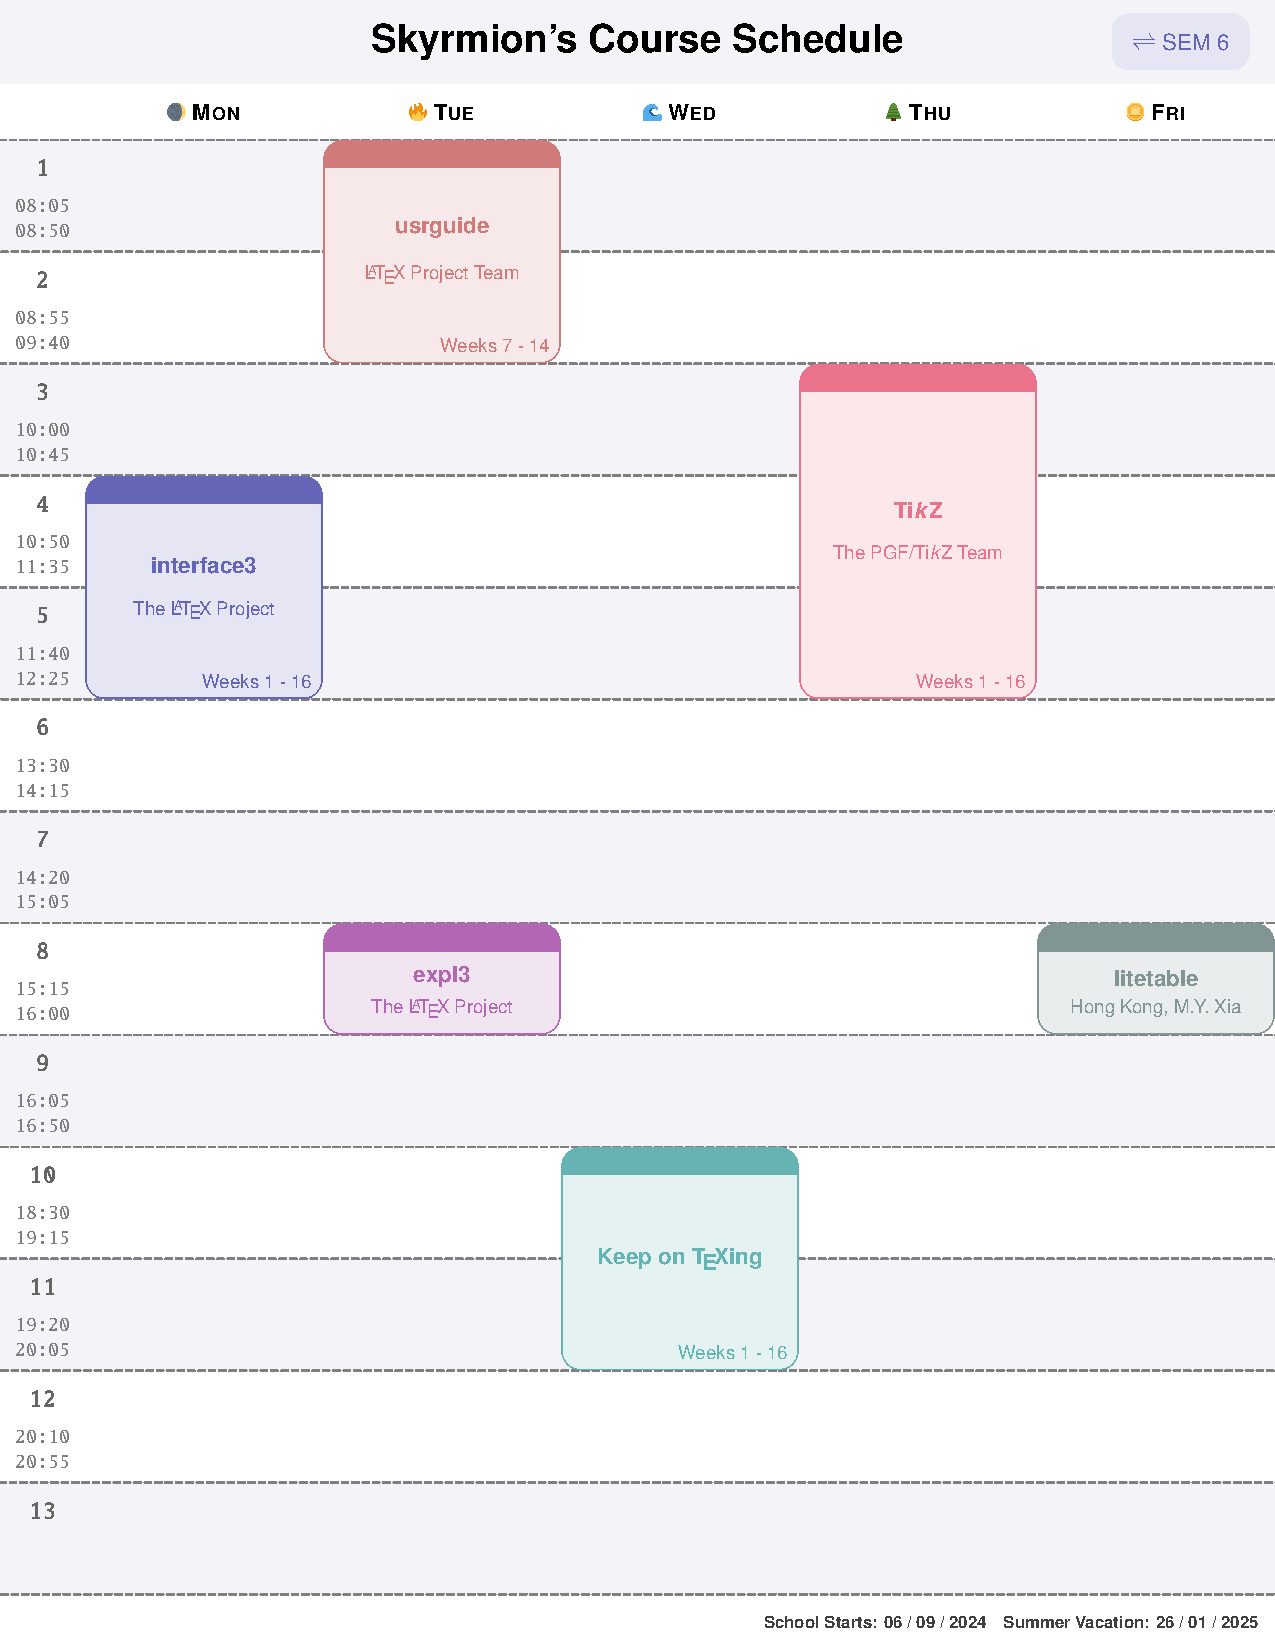
\includepdf[pages = 1]{litetable-demo.pdf}

\end{document}